% FILE: content/07_figures.tex

\section{Illustrative Figures}
\label{sec:figures}

This appendix collects the illustrative TikZ figures used in the Core~1.1
release. Each panel visualises a structural component or level of the
Ontology of Continua (OC). All figures are generated from standalone
TikZ snippets in the \texttt{figures/} directory.

\begin{figure}[p]
  \centering
  % FILE: figures/continua_structure.tex
% Structural diagram of a continuum K

\begin{tikzpicture}[node distance=1.4cm,>=latex,thick]

% Main node for K
\node[draw, rounded corners, fill=gray!10, inner sep=8pt] (K) {$K$};

% Components
\node[draw, left=of K, rounded corners, fill=blue!10]  (Omega) {$\Omega(K)$};
\node[draw, right=of K, rounded corners, fill=blue!10] (A)     {$A(K)$};

\node[draw, above=of K, rounded corners, fill=green!10] (P)  {$P(t)$};
\node[draw, below=of K, rounded corners, fill=green!10] (J)  {$J(t)$};

\node[draw, below left=of K, rounded corners, fill=yellow!15] (Theta) {$\Theta(K)$};
\node[draw, below right=of K, rounded corners, fill=yellow!15] (Boundary) {$\partial\Omega(K)$};

\node[draw, above left=of K, rounded corners, fill=red!10] (C) {$C(K)$};
\node[draw, above right=of K, rounded corners, fill=red!10] (k) {$k(t)$};

% Connections
\draw[->] (P) -- (K);
\draw[->] (J) -- (K);
\draw[->] (Omega) -- (K);
\draw[->] (A) -- (K);
\draw[->] (Theta) -- (K);
\draw[->] (Boundary) -- (K);
\draw[->] (C) -- (K);
\draw[->] (k) -- (K);

\end{tikzpicture}

  \caption{Schematic structure of a continuum
           \(K = (\Omega, A, P, J, \Theta, \partial\Omega, C, k)\).}
  \label{fig:continua-structure}
\end{figure}

\begin{figure}[p]
  \centering
  % FILE: figures/axes_thresholds.tex
% Axes and threshold geometry of continua

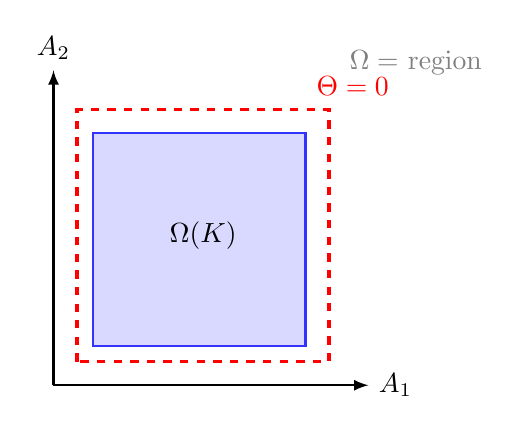
\begin{tikzpicture}[>=latex,thick]

% Axes
\draw[->] (0,0) -- (4,0) node[right] {$A_1$};
\draw[->] (0,0) -- (0,4) node[above] {$A_2$};

% State region Omega
\filldraw[fill=blue!15, draw=blue!80] (0.5,0.5) rectangle (3.2,3.2);
\node at (1.9,1.9) {$\Omega(K)$};

% Threshold boundary
\draw[red, very thick, dashed] (0.3,0.3) rectangle (3.5,3.5);
\node[red] at (3.8,3.8) {$\Theta = 0$};

% Death zone
\node[gray] at (4.6,4.1) {$\Omega = \varnothing$ region};

\end{tikzpicture}

  \caption{Axes and threshold surfaces in the extended state space of a
           continuum.}
  \label{fig:axes-thresholds}
\end{figure}

\begin{figure}[p]
  \centering
  
% FILE: figures/thresholds_taxonomy.tex
% Taxonomy of thresholds

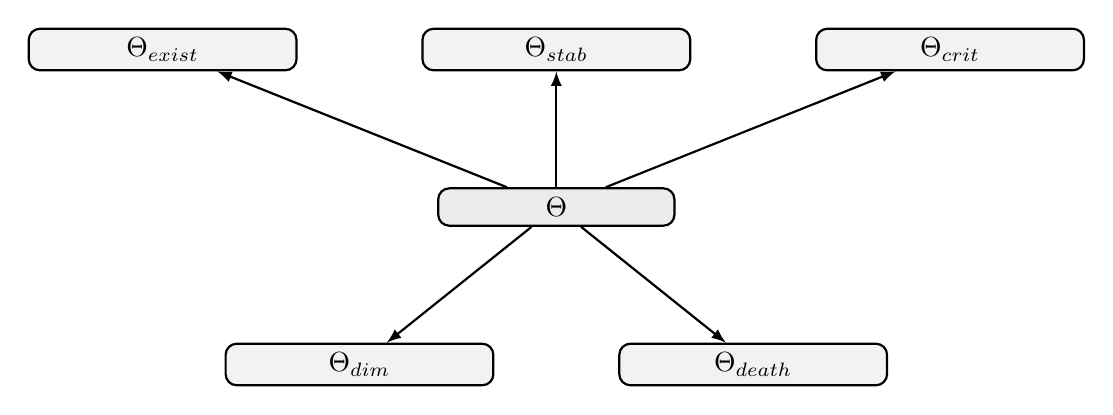
\begin{tikzpicture}[>=latex,thick]
  % Central node
  \node[draw, rounded corners, fill=gray!15, minimum width=3cm] (Theta) at (0,0) {$\Theta$};

  % Children
  \node[draw, rounded corners, fill=gray!10, minimum width=3.4cm] (exist) at (-5, 2) {$\Theta_{\text{exist}}$};
  \node[draw, rounded corners, fill=gray!10, minimum width=3.4cm] (stab)  at ( 0, 2) {$\Theta_{\text{stab}}$};
  \node[draw, rounded corners, fill=gray!10, minimum width=3.4cm] (crit)  at ( 5, 2) {$\Theta_{\text{crit}}$};

  \node[draw, rounded corners, fill=gray!10, minimum width=3.4cm] (dim)   at (-2.5,-2) {$\Theta_{\text{dim}}$};
  \node[draw, rounded corners, fill=gray!10, minimum width=3.4cm] (death) at ( 2.5,-2) {$\Theta_{\text{death}}$};

  % Arrows
  \draw[->] (Theta) -- (exist);
  \draw[->] (Theta) -- (stab);
  \draw[->] (Theta) -- (crit);
  \draw[->] (Theta) -- (dim);
  \draw[->] (Theta) -- (death);
\end{tikzpicture}

  \caption{Taxonomy of thresholds:
           existence, stability, critical, dimensional and death thresholds.}
  \label{fig:thresholds-taxonomy}
\end{figure}

\begin{figure}[p]
  \centering
  % FILE: figures/delta_threshold_k0.tex
% Delta function and threshold in K0

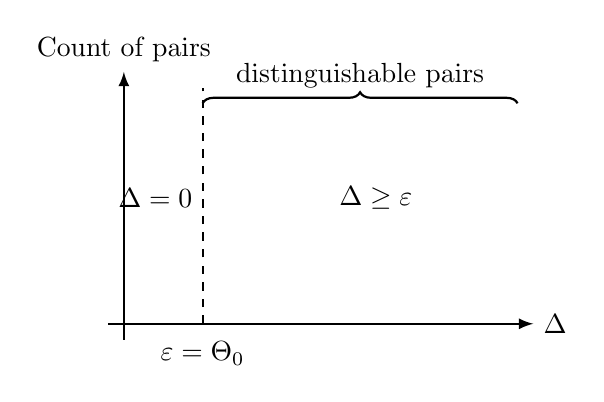
\begin{tikzpicture}[>=latex,thick,scale=1]
  % Axes
  \draw[->] (-0.2,0) -- (5.2,0) node[right] {$\Delta$};
  \draw[->] (0,-0.2) -- (0,3.2) node[above] {Count of pairs};

  % Threshold epsilon line
  \draw[dashed] (1,0) -- (1,3);
  \node[anchor=north] at (1,-0.1) {$\varepsilon=\Theta_0$};

  % Regions
  \node at (0.4,1.6) {$\Delta=0$};
  \node at (3.2,1.6) {$\Delta \geq \varepsilon$};

  \draw[decorate,decoration={brace,amplitude=4pt}] (1,2.8) -- (5,2.8)
    node[midway,anchor=south,yshift=2pt] {distinguishable pairs};
\end{tikzpicture}

  \caption{Structural difference and minimal threshold \texorpdfstring{\(\Theta_0\)}{\Theta_0} at level
           \texorpdfstring{\(K_0\)}{K_0}.}
  \label{fig:delta-threshold-k0}
\end{figure}

\begin{figure}[p]
  \centering
  % FILE: figures/k0_to_k1_transition.tex
% Transition from K0 to K1

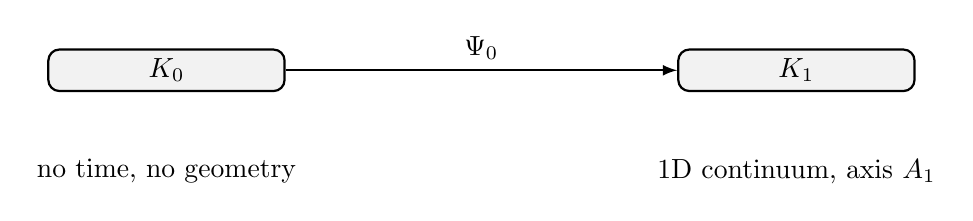
\begin{tikzpicture}[>=latex,thick]
  % K0
  \node[draw, rounded corners, fill=gray!10, minimum width=3cm] (K0) at (-4,0) {$K_0$};
  \node[anchor=north] at (-4,-1.0) {no time, no geometry};

  % K1
  \node[draw, rounded corners, fill=gray!10, minimum width=3cm] (K1) at (4,0) {$K_1$};
  \node[anchor=north] at (4,-1.0) {1D continuum, axis $A_1$};

  % Arrow with label
  \draw[->] (K0) -- node[above] {$\Psi_0$} (K1);
\end{tikzpicture}

  \caption{Schematic of the transition \(\Psi_{0\to 1}\) from the substrate
           \(K_0\) to the first continuum \(K_1\).}
  \label{fig:k0-k1-transition}
\end{figure}

\begin{figure}[p]
  \centering
  % FILE: figures/levels_hierarchy.tex
% Vertical hierarchy K0--K10

\begin{tikzpicture}[node distance=1.1cm,>=latex,thick]

% List levels
\node[draw, fill=gray!15, rounded corners] (K0) {$K_0$};
\node[draw, fill=gray!15, rounded corners, below=of K0] (K1) {$K_1$};
\node[draw, fill=gray!15, rounded corners, below=of K1] (K2) {$K_2$};
\node[draw, fill=gray!15, rounded corners, below=of K2] (K3) {$K_3$};
\node[draw, fill=gray!15, rounded corners, below=of K3] (K4) {$K_4$};
\node[draw, fill=gray!15, rounded corners, below=of K4] (K5) {$K_5$};
\node[draw, fill=gray!15, rounded corners, below=of K5] (K6) {$K_6$};
\node[draw, fill=gray!15, rounded corners, below=of K6] (K7) {$K_7$};
\node[draw, fill=gray!15, rounded corners, below=of K7] (K8) {$K_8$};
\node[draw, fill=gray!15, rounded corners, below=of K8] (K9) {$K_9$};
\node[draw, fill=gray!15, rounded corners, below=of K9] (K10) {$K_{10}$};

% Arrows
\foreach \i/\j in {K0/K1, K1/K2, K2/K3, K3/K4, K4/K5, K5/K6, K6/K7, K7/K8, K8/K9, K9/K10}
{
    \draw[->] (\i) -- (\j);
}

\end{tikzpicture}

  \caption{Vertical hierarchy of continua from \texorpdfstring{\(K_0\)}{K_0} to \(K_{10}\).}
  \label{fig:levels-hierarchy}
\end{figure}

\begin{figure}[p]
  \centering
  % FILE: figures/potential_landscape.tex
% Schematic potential landscape with thresholds

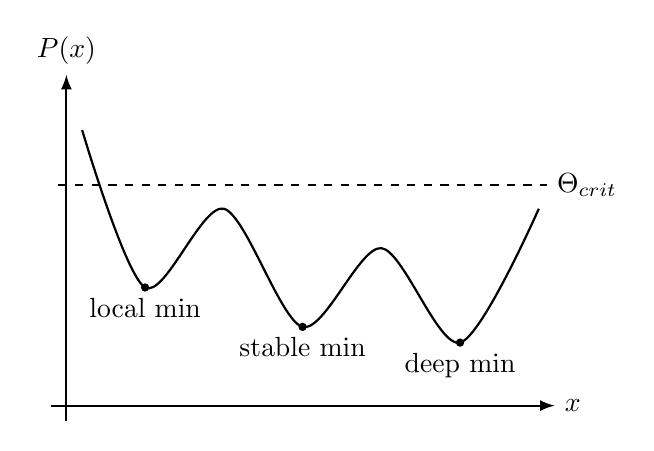
\begin{tikzpicture}[>=latex,thick,scale=1]
  % Axes
  \draw[->] (-0.2,0) -- (6.2,0) node[right] {$x$};
  \draw[->] (0,-0.2) -- (0,4.2) node[above] {$P(x)$};

  % Potential curve (hand-drawn with a few points)
  \draw[smooth,thick]
    plot coordinates {
      (0.2,3.5)
      (1.0,1.5)
      (2.0,2.5)
      (3.0,1.0)
      (4.0,2.0)
      (5.0,0.8)
      (6.0,2.5)
    };

  % Threshold line
  \draw[dashed] (-0.1,2.8) -- (6.1,2.8);
  \node[anchor=west] at (6.1,2.8) {$\Theta_{\text{crit}}$};

  % Local minima labels
  \fill (1.0,1.5) circle (1.5pt);
  \node[below] at (1.0,1.5) {local min};

  \fill (3.0,1.0) circle (1.5pt);
  \node[below] at (3.0,1.0) {stable min};

  \fill (5.0,0.8) circle (1.5pt);
  \node[below] at (5.0,0.8) {deep min};
\end{tikzpicture}


  \caption{Illustrative potential landscape and flows \(J(t)\) on a continuum.}
  \label{fig:potential-landscape}
\end{figure}

\begin{figure}[p]
  \centering
  % FILE: figures/evolution_operator.tex
% Evolution operator E: K(t) -> K(t+dt)

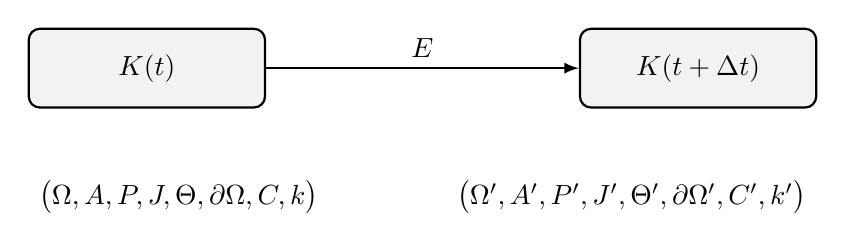
\begin{tikzpicture}[>=latex,thick]
  \node[draw, rounded corners, fill=gray!10, minimum width=3cm, minimum height=1cm] (Kt)   at (0,0) {$K(t)$};
  \node[draw, rounded corners, fill=gray!10, minimum width=3cm, minimum height=1cm] (Ktdt) at (7,0) {$K(t+\Delta t)$};

  \draw[->] (Kt) -- node[above] {$E$} (Ktdt);

  % Annotations
  \node[anchor=north west] at (-1.5,-1.3) {$\big(\Omega,A,P,J,\Theta,\partial\Omega,C,k\big)$};
  \node[anchor=north east] at (8.5,-1.3) {$\big(\Omega',A',P',J',\Theta',\partial\Omega',C',k'\big)$};
\end{tikzpicture}



  \caption{Schematic action of the evolution operator
           \(E : K(t) \mapsto K(t+dt)\).}
  \label{fig:evolution-operator}
\end{figure}

\begin{figure}[p]
  \centering
  % FILE: figures/birth_life_death.tex
% Birth, life and death of a continuum

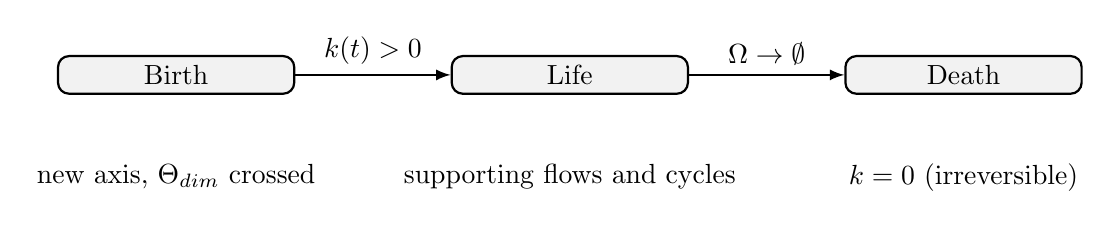
\begin{tikzpicture}[>=latex,thick]
  % States
  \node[draw, rounded corners, fill=gray!10, minimum width=3cm] (birth) at (0,0) {Birth};
  \node[draw, rounded corners, fill=gray!10, minimum width=3cm] (life)  at (5,0) {Life};
  \node[draw, rounded corners, fill=gray!10, minimum width=3cm] (death) at (10,0) {Death};

  % Arrows
  \draw[->] (birth) -- node[above] {$k(t)>0$} (life);
  \draw[->] (life)  -- node[above] {$\Omega \rightarrow \emptyset$} (death);

  % Additional labels
  \node[anchor=north] at (0,-1.0) {new axis, $\Theta_{\text{dim}}$ crossed};
  \node[anchor=north] at (5,-1.0) {supporting flows and cycles};
  \node[anchor=north] at (10,-1.0) {$k=0$ (irreversible)};
\end{tikzpicture}

  \caption{Birth, life and death of a continuum in terms of the state space
           \texorpdfstring{\(\Omega\)}{\Omega}, cycles \texorpdfstring{\(C\)}{C} and the measure \(k(t)\).}
  \label{fig:birth-life-death}
\end{figure}

\begin{figure}[p]
  \centering
  % FILE: figures/percolation_diagram.tex
% Percolation clusters schematic

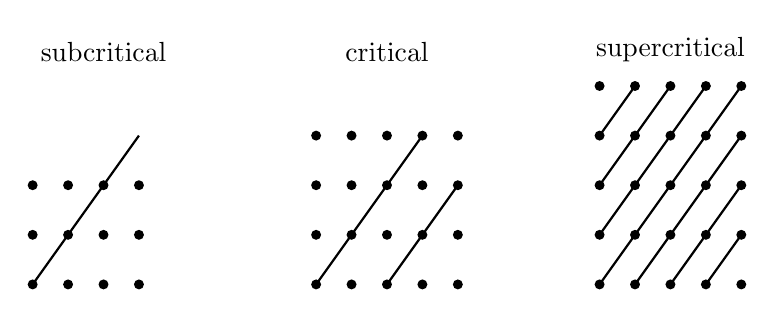
\begin{tikzpicture}[>=latex,thick,scale=0.9]
  % Subcritical
  \node[anchor=south] at (-4,3) {subcritical};
  \foreach \x in {-5,-4.5,-4,-3.5}
    \foreach \y in {0,0.7,1.4}
      \fill (\x,\y) circle (2pt);

  \foreach \x/\y in {-5/0, -4.5/0.7, -4/1.4}
    \draw (\x,\y) -- ++(0.5,0.7);

  % Critical
  \node[anchor=south] at (0,3) {critical};
  \foreach \x in {-1, -0.5, 0, 0.5, 1}
    \foreach \y in {0,0.7,1.4,2.1}
      \fill (\x,\y) circle (2pt);

  \draw (-1,0) -- (-0.5,0.7) -- (0,1.4) -- (0.5,2.1);
  \draw (0,0) -- (0.5,0.7) -- (1,1.4);

  % Supercritical
  \node[anchor=south] at (4,3) {supercritical};
  \foreach \x in {3,3.5,4,4.5,5}
    \foreach \y in {0,0.7,1.4,2.1,2.8}
      \fill (\x,\y) circle (2pt);

  \foreach \x in {3,3.5,4,4.5}
    \foreach \y in {0,0.7,1.4,2.1}
      \draw (\x,\y) -- ++(0.5,0.7);
\end{tikzpicture}


  \caption{Percolation--type transition at level \texorpdfstring{\(K_2\)}{K_2}.}
  \label{fig:percolation}
\end{figure}

\begin{figure}[p]
  \centering
  % FILE: figures/bkt_transition.tex
% BKT-like vortex/antivortex schematic

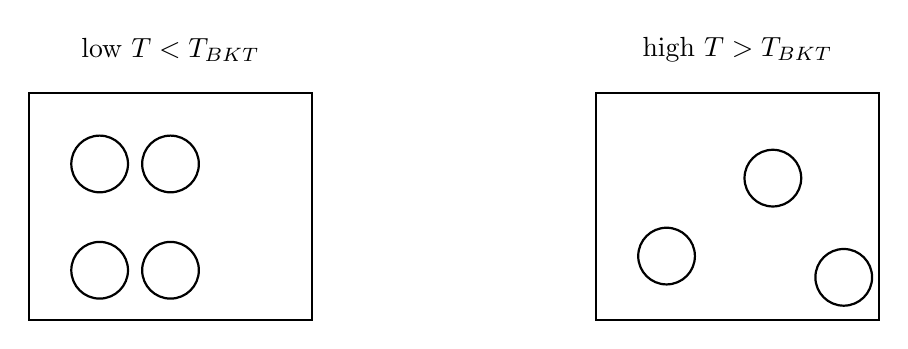
\begin{tikzpicture}[>=latex,thick,scale=0.9]
  % Low T panel
  \node[anchor=south] at (-4,3.3) {low $T<T_{\text{BKT}}$};
  \draw (-6,-0.2) rectangle (-2,3);

  % Bound vortex-antivortex pairs
  \draw[->] (-5,0.5) circle (0.4);
  \draw[<-] (-4,0.5) circle (0.4);
  \draw[->] (-5,2.0) circle (0.4);
  \draw[<-] (-4,2.0) circle (0.4);

  % High T panel
  \node[anchor=south] at (4,3.3) {high $T>T_{\text{BKT}}$};
  \draw (2,-0.2) rectangle (6,3);

  % Free vortices
  \draw[->] (3,0.7) circle (0.4);
  \draw[->] (4.5,1.8) circle (0.4);
  \draw[<-] (5.5,0.4) circle (0.4);
\end{tikzpicture}

  \caption{BKT--type transition as an example of threshold--governed emergence
           of a new topological axis.}
  \label{fig:bkt-transition}
\end{figure}

\begin{figure}[p]
  \centering
  % FILE: figures/qubit_bloch_sphere.tex
% Bloch sphere schematic

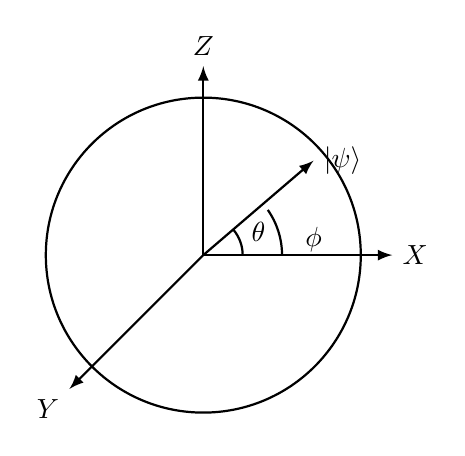
\begin{tikzpicture}[>=latex,thick,scale=1]
  % Circle
  \draw (0,0) circle (2);

  % Axes
  \draw[->] (0,0) -- (0,2.4) node[above] {$Z$};
  \draw[->] (0,0) -- (2.4,0) node[right] {$X$};
  \draw[->] (0,0) -- (-1.7,-1.7) node[below left] {$Y$};

  % State vector
  \draw[->,thick] (0,0) -- (1.4,1.2);
  \node[anchor=west] at (1.4,1.2) {$|\psi\rangle$};

  % Angles
  \draw (0.5,0) arc (0:40:0.5);
  \node at (0.7,0.3) {$\theta$};

  \draw (1.0,0) arc (0:35:1.0);
  \node at (1.4,0.2) {$\phi$};
\end{tikzpicture}

  \caption{Illustrative Bloch sphere diagram for quantum two--level systems.}
  \label{fig:bloch-sphere}
\end{figure}

\begin{figure}[p]
  \centering
  
% FILE: figures/raf_network.tex
% RAF network schematic

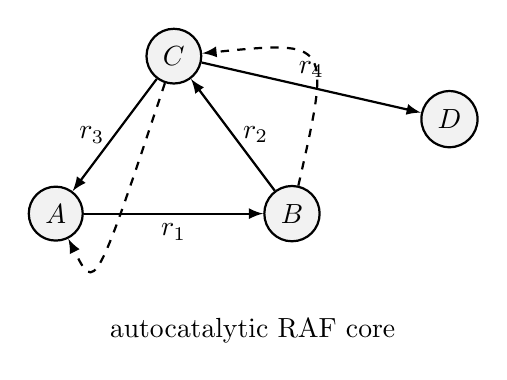
\begin{tikzpicture}[>=latex,thick,scale=1]
  % Molecules
  \node[draw, circle, fill=gray!10] (A) at (0,0) {$A$};
  \node[draw, circle, fill=gray!10] (B) at (3,0) {$B$};
  \node[draw, circle, fill=gray!10] (C) at (1.5,2) {$C$};
  \node[draw, circle, fill=gray!10] (D) at (5,1.2) {$D$};

  % Reactions
  \draw[->] (A) -- (B) node[midway,below] {$r_1$};
  \draw[->] (B) -- (C) node[midway,right] {$r_2$};
  \draw[->] (C) -- (A) node[midway,left] {$r_3$};
  \draw[->] (C) -- (D) node[midway,above] {$r_4$};

  % Catalytic edges
  \draw[dashed,->] (C) .. controls (0.5,-1.0) .. (A);
  \draw[dashed,->] (B) .. controls (3.5,2.2) .. (C);

  \node[anchor=north] at (2.5,-1.2) {autocatalytic RAF core};
\end{tikzpicture}

  \caption{RAF network as a chemical continuum at level \texorpdfstring{\(K_3\)}{K_3}.}
  \label{fig:raf-network}
\end{figure}

\begin{figure}[p]
  \centering
  % FILE: figures/catalytic_paths.tex
% Catalytic vs non-catalytic reaction paths

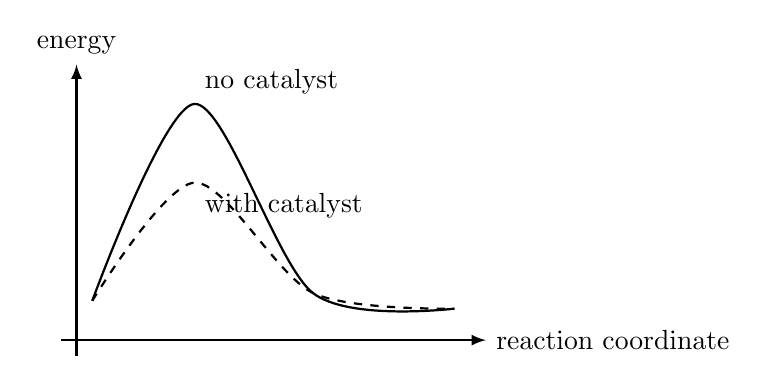
\begin{tikzpicture}[>=latex,thick,scale=1]
  % Axes
  \draw[->] (-0.2,0) -- (5.2,0) node[right] {reaction coordinate};
  \draw[->] (0,-0.2) -- (0,3.5) node[above] {energy};

  % Uncatalyzed path
  \draw[smooth,thick]
    plot coordinates {
      (0.2,0.5)
      (1.5,3.0)
      (3.0,0.6)
      (4.8,0.4)
    };
  \node[anchor=south west] at (1.5,3.0) {no catalyst};

  % Catalyzed path
  \draw[smooth,thick,dashed]
    plot coordinates {
      (0.2,0.5)
      (1.5,2.0)
      (3.0,0.6)
      (4.8,0.4)
    };
  \node[anchor=north west] at (1.5,2.0) {with catalyst};
\end{tikzpicture}


  \caption{Catalytic paths and supporting flows in a reaction network.}
  \label{fig:catalytic-paths}
\end{figure}

\begin{figure}[p]
  \centering
  % FILE: figures/membrane_closure.tex
% Membrane closure schematic (vesicle formation)

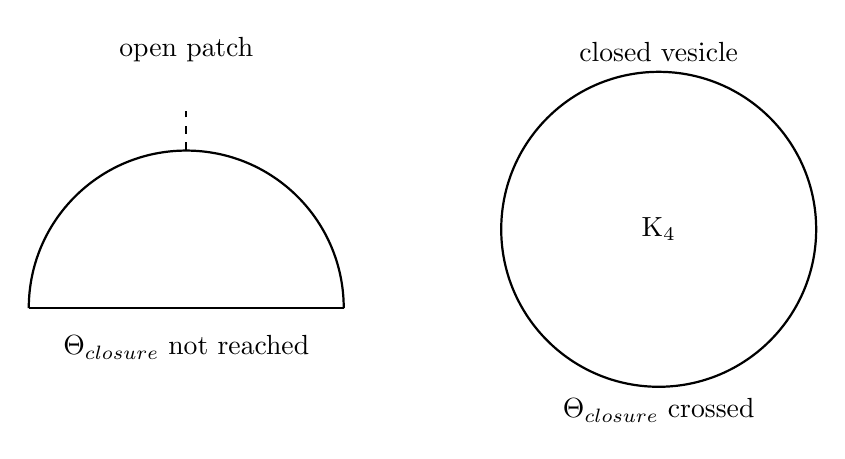
\begin{tikzpicture}[>=latex,thick,scale=1]
  % Open patch
  \node[anchor=south] at (-3,3.0) {open patch};
  \draw (-5,0) -- (-1,0);
  \draw (-5,0) arc (180:0:2);
  % "gap" at top
  \draw[dashed] (-3,2.0) -- (-3,2.5);
  \node at (-3,-0.5) {$\Theta_{\text{closure}}$ not reached};

  % Closed vesicle
  \node[anchor=south] at (3,3.0) {closed vesicle};
  \draw (3,1.0) circle (2.0);
  \node at (3,1.0) {K$_4$};
  \node at (3,-1.3) {$\Theta_{\text{closure}}$ crossed};
\end{tikzpicture}


  \caption{Membrane closure and emergence of a protocellular boundary
           at level \texorpdfstring{\(K_4\)}{K_4}.}
  \label{fig:membrane-closure}
\end{figure}

\begin{figure}[p]
  \centering
  % FILE: figures/gradient_osmosis_tension.tex
% Gradients and osmotic tension

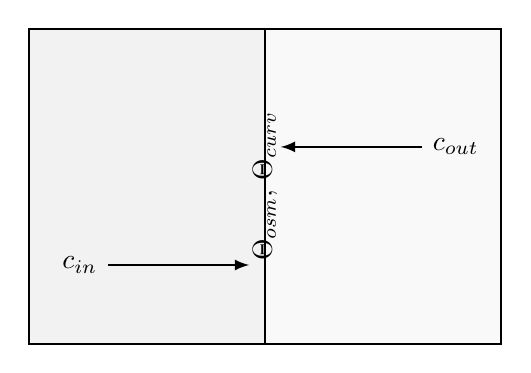
\begin{tikzpicture}[>=latex,thick,scale=1]
  % Membrane
  \draw[thick] (0,0) -- (0,4);

  % Left compartment (inside)
  \node at (-1.5,3.5) {inside};
  \draw[fill=gray!10] (-3,0) rectangle (0,4);

  % Right compartment (outside)
  \node at (1.5,3.5) {outside};
  \draw[fill=gray!5] (0,0) rectangle (3,4);

  % Concentration gradients (arrows)
  \draw[->] (-2.0,1.0) -- (-0.2,1.0);
  \node[anchor=east] at (-2.0,1.0) {$c_{\text{in}}$};

  \draw[->] (2.0,2.5) -- (0.2,2.5);
  \node[anchor=west] at (2.0,2.5) {$c_{\text{out}}$};

  % Tension label
  \node[rotate=90] at (0,2.0) {$\Theta_{\text{osm}}$, $\Theta_{\text{curv}}$};
\end{tikzpicture}

  \caption{Osmotic gradients, membrane tension and structural thresholds
           in protocells.}
  \label{fig:gradient-osmosis-tension}
\end{figure}

\begin{figure}[p]
  \centering
  % FILE: figures/vesicle_flickering.tex
% Vesicle flickering regime schematic

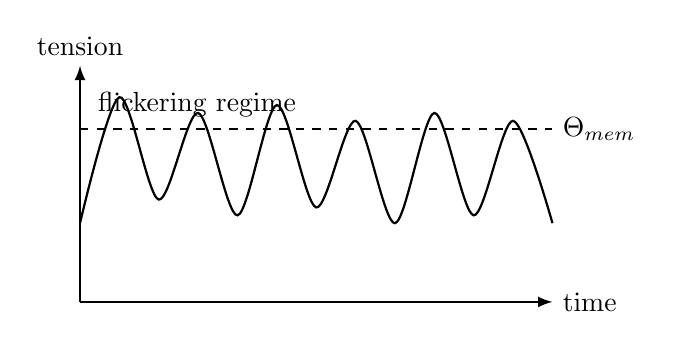
\begin{tikzpicture}[>=latex,thick,scale=1]
  % Time axis
  \draw[->] (0,0) -- (6,0) node[right] {time};
  \draw[->] (0,0) -- (0,3) node[above] {tension};

  % Threshold
  \draw[dashed] (0,2.2) -- (6,2.2);
  \node[anchor=west] at (6,2.2) {$\Theta_{\text{mem}}$};

  % Oscillatory tension
  \draw[smooth,thick]
    plot coordinates {
      (0.0,1.0)
      (0.5,2.6)
      (1.0,1.3)
      (1.5,2.4)
      (2.0,1.1)
      (2.5,2.5)
      (3.0,1.2)
      (3.5,2.3)
      (4.0,1.0)
      (4.5,2.4)
      (5.0,1.1)
      (5.5,2.3)
      (6.0,1.0)
    };

  \node[anchor=north west] at (0.1,2.8) {flickering regime};
\end{tikzpicture}

  \caption{Vesicle flickering regime near curvature and osmotic thresholds.}
  \label{fig:vesicle-flickering}
\end{figure}

\begin{figure}[p]
  \centering
  % FILE: figures/dv_propagation_membrane.tex
% Spatial propagation of Delta V along membrane

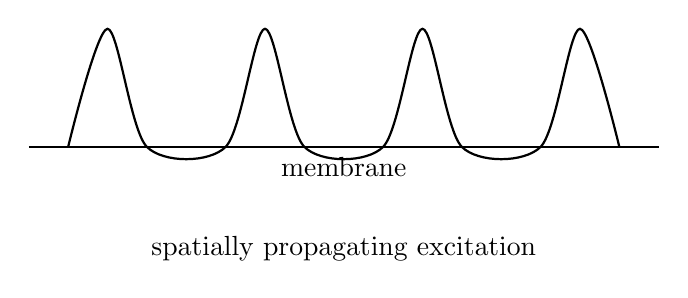
\begin{tikzpicture}[>=latex,thick,scale=1]
  % Membrane line
  \draw[thick] (0,0) -- (8,0);
  \node[anchor=north] at (4,0) {membrane};

  % Voltage peaks
  \draw[smooth,thick]
    plot coordinates {
      (0.5,0)
      (1.0,1.5)
      (1.5,0)
      (2.5,0)
      (3.0,1.5)
      (3.5,0)
      (4.5,0)
      (5.0,1.5)
      (5.5,0)
      (6.5,0)
      (7.0,1.5)
      (7.5,0)
    };

  \node[anchor=north] at (4,-1.0) {spatially propagating excitation};
\end{tikzpicture}


  \caption{Propagation of membrane potential \texorpdfstring{\(\Delta V\)}{\Delta V} along a boundary.}
  \label{fig:dv-propagation-membrane}
\end{figure}

\begin{figure}[p]
  \centering
  % FILE: figures/ion_channel_states.tex
% Ion channel state diagram

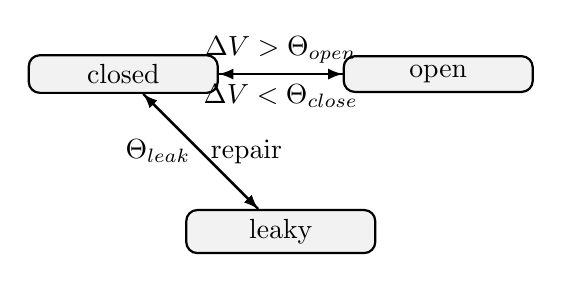
\begin{tikzpicture}[>=latex,thick,scale=1]
  % States
  \node[draw, rounded corners, fill=gray!10, minimum width=2.4cm] (closed) at (0,0) {closed};
  \node[draw, rounded corners, fill=gray!10, minimum width=2.4cm] (open)   at (4,0) {open};
  \node[draw, rounded corners, fill=gray!10, minimum width=2.4cm] (leaky)  at (2,-2) {leaky};

  % Transitions
  \draw[->] (closed) -- node[above] {$\Delta V>\Theta_{\text{open}}$} (open);
  \draw[->] (open)   -- node[below] {$\Delta V<\Theta_{\text{close}}$} (closed);
  \draw[->] (closed) -- node[left] {$\Theta_{\text{leak}}$} (leaky);
  \draw[->] (leaky)  -- node[right] {repair} (closed);
\end{tikzpicture}


  \caption{Ion channel states and excitation thresholds at level \texorpdfstring{\(K_5\)}{K_5}.}
  \label{fig:ion-channel-states}
\end{figure}

\begin{figure}[p]
  \centering
  % FILE: figures/proto_spike.tex
% Proto-spike voltage trace

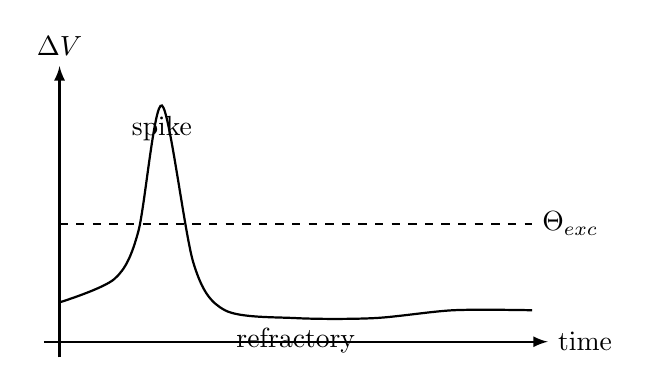
\begin{tikzpicture}[>=latex,thick,scale=1]
  % Axes
  \draw[->] (-0.2,0) -- (6.2,0) node[right] {time};
  \draw[->] (0,-0.2) -- (0,3.5) node[above] {$\Delta V$};

  % Threshold
  \draw[dashed] (0,1.5) -- (6,1.5);
  \node[anchor=west] at (6,1.5) {$\Theta_{\text{exc}}$};

  % Proto-spike
  \draw[smooth,thick]
    plot coordinates {
      (0.0,0.5)
      (0.7,0.8)
      (1.0,1.4)
      (1.3,3.0)
      (1.7,1.0)
      (2.1,0.4)
      (3.0,0.3)
      (4.0,0.3)
      (5.0,0.4)
      (6.0,0.4)
    };

  \node[anchor=north] at (1.3,3.0) {spike};
  \node[anchor=north] at (3.0,0.3) {refractory};
\end{tikzpicture}


  \caption{Proto--spike dynamics as a minimal excitatory cycle.}
  \label{fig:proto-spike}
\end{figure}

\begin{figure}[p]
  \centering
  % FILE: figures/cognitive_state_space.tex
% Cognitive state space with stable region

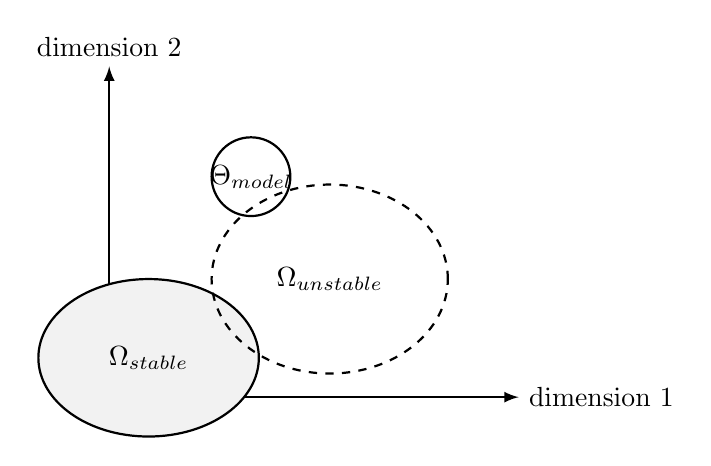
\begin{tikzpicture}[>=latex,thick,scale=1]
  % Axes
  \draw[->] (-0.2,0) -- (5.2,0) node[right] {dimension 1};
  \draw[->] (0,-0.2) -- (0,4.2) node[above] {dimension 2};

  % Stable region
  \draw[fill=gray!10] (0.5,0.5) ellipse (1.4 and 1.0);
  \node at (0.5,0.5) {$\Omega_{\text{stable}}$};

  % Unstable region
  \draw[dashed] (2.8,1.5) ellipse (1.5 and 1.2);
  \node at (2.8,1.5) {$\Omega_{\text{unstable}}$};

  % Threshold contour
  \draw[thick] (1.8,2.8) circle (0.5);
  \node at (1.8,2.8) {$\Theta_{\text{model}}$};
\end{tikzpicture}


  \caption{Schematic cognitive state space and binding axes at level \texorpdfstring{\(K_6\)}{K_6}.}
  \label{fig:cognitive-state-space}
\end{figure}

\begin{figure}[p]
  \centering
  % FILE: figures/binding_space.tex
% Cognitive binding space schematic

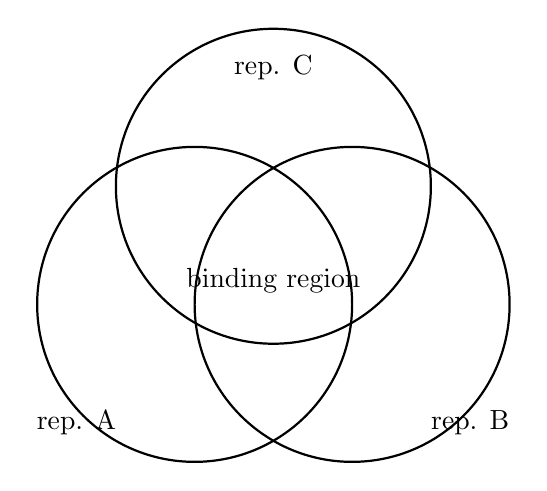
\begin{tikzpicture}[>=latex,thick,scale=1]
  % Overlapping circles
  \draw (0,0) circle (2);
  \draw (2,0) circle (2);
  \draw (1,1.5) circle (2);

  \node at (-1.5,-1.5) {rep. A};
  \node at (3.5,-1.5) {rep. B};
  \node at (1,3.0) {rep. C};

  \node at (1,0.3) {binding region};
\end{tikzpicture}


  \caption{Binding space for cognitive continua and associated thresholds.}
  \label{fig:binding-space}
\end{figure}

\begin{figure}[p]
  \centering
  % FILE: figures/institutional_cycles.tex
% Institutional cycles in a social continuum

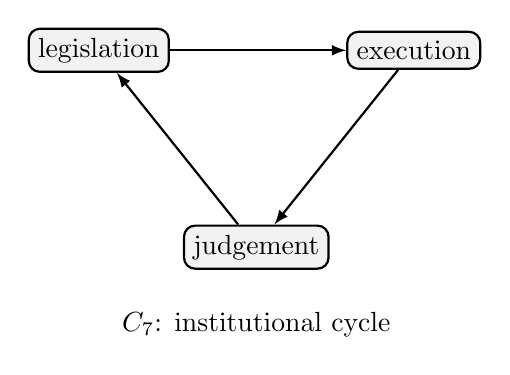
\begin{tikzpicture}[>=latex,thick,scale=1]
  % Cycle nodes
  \node[draw, rounded corners, fill=gray!10] (Leg) at (0,0) {legislation};
  \node[draw, rounded corners, fill=gray!10] (Exec) at (4,0) {execution};
  \node[draw, rounded corners, fill=gray!10] (Jud) at (2,-2.5) {judgement};

  % Cycle arrows
  \draw[->] (Leg) -- (Exec);
  \draw[->] (Exec) -- (Jud);
  \draw[->] (Jud) -- (Leg);

  \node[anchor=north] at (2,-3.2) {$C_7$: institutional cycle};
\end{tikzpicture}

  \caption{Institutional cycles and social flows at level \texorpdfstring{\(K_7\)}{K_7}.}
  \label{fig:institutional-cycles}
\end{figure}

\begin{figure}[p]
  \centering
  
% FILE: figures/trust_threshold.tex
% Trust threshold in a social continuum

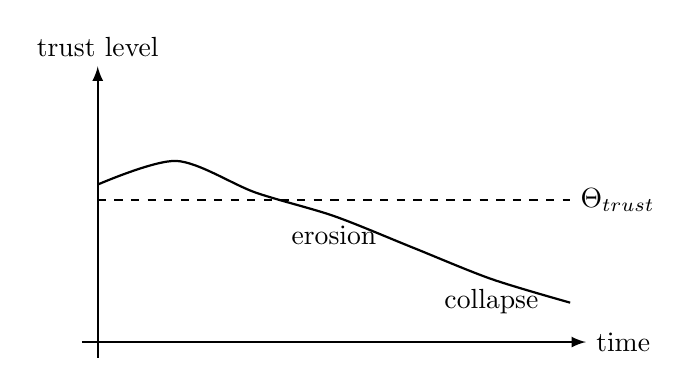
\begin{tikzpicture}[>=latex,thick,scale=1]
  % Axes
  \draw[->] (-0.2,0) -- (6.2,0) node[right] {time};
  \draw[->] (0,-0.2) -- (0,3.5) node[above] {trust level};

  % Threshold
  \draw[dashed] (0,1.8) -- (6,1.8);
  \node[anchor=west] at (6,1.8) {$\Theta_{\text{trust}}$};

  % Trust dynamics
  \draw[smooth,thick]
    plot coordinates {
      (0.0,2.0)
      (1.0,2.3)
      (2.0,1.9)
      (3.0,1.6)
      (4.0,1.2)
      (5.0,0.8)
      (6.0,0.5)
    };

  \node[anchor=north] at (3.0,1.6) {erosion};
  \node[anchor=north] at (5.0,0.8) {collapse};
\end{tikzpicture}


  \caption{Trust thresholds and collapse of social continuumness.}
  \label{fig:trust-threshold}
\end{figure}

\begin{figure}[p]
  \centering
  % FILE: figures/civilization_energy_cycles.tex
% Civilizational energy and infrastructure cycles

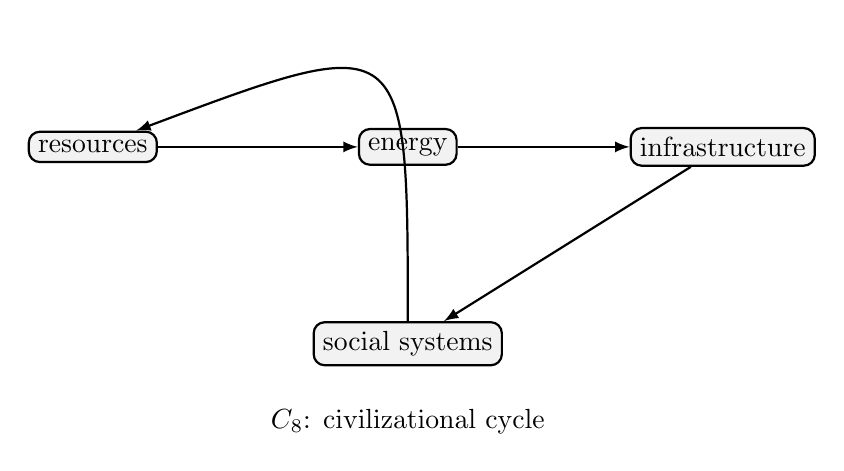
\begin{tikzpicture}[>=latex,thick,scale=1]
  % Nodes
  \node[draw, rounded corners, fill=gray!10] (Res) at (0,0) {resources};
  \node[draw, rounded corners, fill=gray!10] (Energy) at (4,0) {energy};
  \node[draw, rounded corners, fill=gray!10] (Infra) at (8,0) {infrastructure};
  \node[draw, rounded corners, fill=gray!10] (Soc) at (4,-2.5) {social systems};

  % Arrows
  \draw[->] (Res) -- (Energy);
  \draw[->] (Energy) -- (Infra);
  \draw[->] (Infra) -- (Soc);
  \draw[->] (Soc) .. controls (4,1.5) .. (Res);

  \node[anchor=north] at (4,-3.2) {$C_8$: civilizational cycle};
\end{tikzpicture}


  \caption{Civilizational energy and infrastructure cycles at level \texorpdfstring{\(K_8\)}{K_8}.}
  \label{fig:civilization-energy-cycles}
\end{figure}

\begin{figure}[p]
  \centering
  % FILE: figures/technological_layers_m8.tex
% Technological layers as embedding space M8

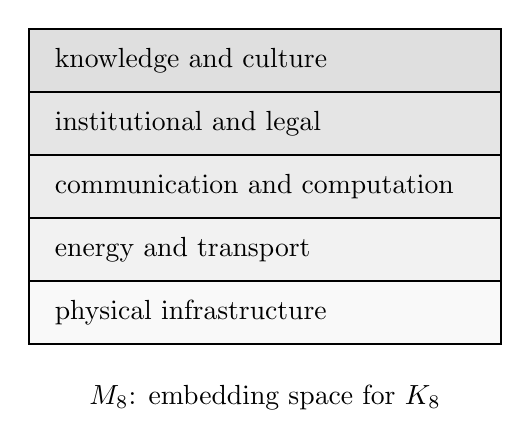
\begin{tikzpicture}[>=latex,thick,scale=1]
  % Layers (stacked rectangles)
  \draw[fill=gray!5] (0,0) rectangle (6,0.8);
  \node[anchor=west] at (0.2,0.4) {physical infrastructure};

  \draw[fill=gray!10] (0,0.8) rectangle (6,1.6);
  \node[anchor=west] at (0.2,1.2) {energy and transport};

  \draw[fill=gray!15] (0,1.6) rectangle (6,2.4);
  \node[anchor=west] at (0.2,2.0) {communication and computation};

  \draw[fill=gray!20] (0,2.4) rectangle (6,3.2);
  \node[anchor=west] at (0.2,2.8) {institutional and legal};

  \draw[fill=gray!25] (0,3.2) rectangle (6,4.0);
  \node[anchor=west] at (0.2,3.6) {knowledge and culture};

  \node[anchor=north] at (3,-0.4) {$M_8$: embedding space for $K_8$};
\end{tikzpicture}

  \caption{Technological layers and embedding spaces for civilizational
           continua.}
  \label{fig:technological-layers-m8}
\end{figure}

\begin{figure}[p]
  \centering
  
% FILE: figures/theory_graph.tex
% Graph of theories in K9

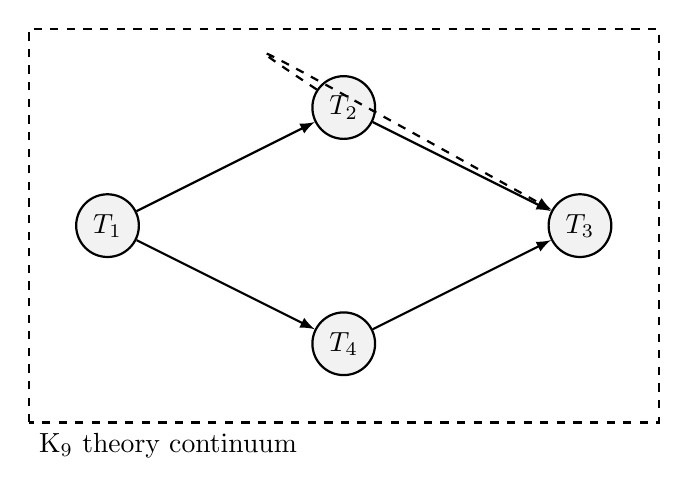
\begin{tikzpicture}[>=latex,thick,scale=1]
  % Theory nodes
  \node[draw, circle, fill=gray!10] (T1) at (0,0) {$T_1$};
  \node[draw, circle, fill=gray!10] (T2) at (3,1.5) {$T_2$};
  \node[draw, circle, fill=gray!10] (T3) at (6,0) {$T_3$};
  \node[draw, circle, fill=gray!10] (T4) at (3,-1.5) {$T_4$};

  % Edges
  \draw[->] (T1) -- (T2);
  \draw[->] (T2) -- (T3);
  \draw[->] (T1) -- (T4);
  \draw[->] (T4) -- (T3);
  \draw[dashed,->] (T2) .. controls (1.5,2.5) .. (T3);

  % Zones
  \draw[dashed] (-1.0,-2.5) rectangle (7.0,2.5);
  \node[anchor=north west] at (-1.0,-2.5) {K$_9$ theory continuum};
\end{tikzpicture}


  \caption{Graph of theories as a continuum at level \texorpdfstring{\(K_9\)}{K_9}.}
  \label{fig:theory-graph}
\end{figure}

\begin{figure}[p]
  \centering
  % FILE: figures/representation_flow_graph.tex
% Representation and information flow graph

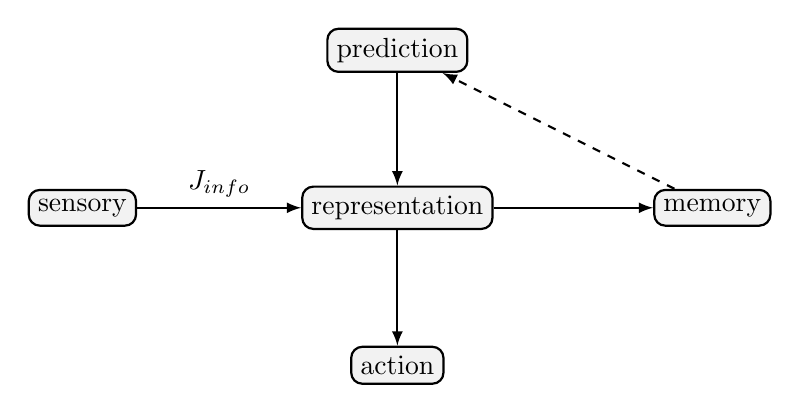
\begin{tikzpicture}[>=latex,thick,scale=1]
  % Nodes
  \node[draw, rounded corners, fill=gray!10] (Sens) at (0,0) {sensory};
  \node[draw, rounded corners, fill=gray!10] (Rep)  at (4,0) {representation};
  \node[draw, rounded corners, fill=gray!10] (Mem)  at (8,0) {memory};

  \node[draw, rounded corners, fill=gray!10] (Act)  at (4,-2) {action};
  \node[draw, rounded corners, fill=gray!10] (Pred) at (4,2) {prediction};

  % Edges
  \draw[->] (Sens) -- node[above] {$J_{\text{info}}$} (Rep);
  \draw[->] (Rep)  -- (Mem);
  \draw[->] (Rep)  -- (Act);
  \draw[->] (Pred) -- (Rep);
  \draw[->,dashed] (Mem) -- (Pred);
\end{tikzpicture}

  \caption{Flows between representations, models and data in \texorpdfstring{\(K_9\)}{K_9}.}
  \label{fig:representation-flow-graph}
\end{figure}

\begin{figure}[p]
  \centering
  % FILE: figures/metatheory_k10_selfreference.tex
% K10 meta-theory self-reference schematic

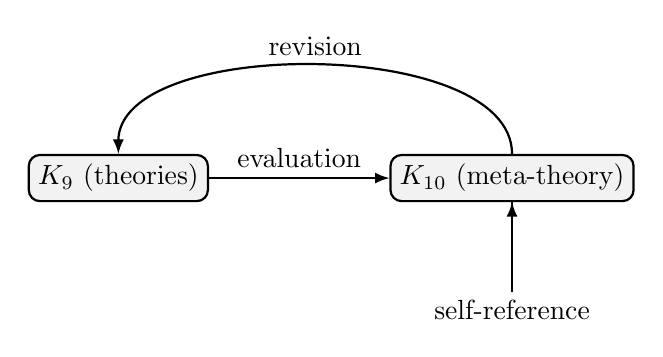
\begin{tikzpicture}[>=latex,thick,scale=1]
  % Nodes
  \node[draw, rounded corners, fill=gray!10] (K9) at (0,0) {$K_9$ (theories)};
  \node[draw, rounded corners, fill=gray!10] (K10) at (5,0) {$K_{10}$ (meta-theory)};

  % Arrows
  \draw[->] (K9) -- node[above] {evaluation} (K10);
  \draw[->] (K10) .. controls (5,1.8) and (0,1.8) .. node[above] {revision} (K9);
  \draw[->] (K10) .. controls (5,-1.8) and (5,-1.8) .. node[below] {self-reference} (K10);
\end{tikzpicture}






  \caption{Self--referential structure of meta--theoretical continua at
           level \(K_{10}\).}
  \label{fig:metatheory-k10-selfreference}
\end{figure}
